It should be apparent at this point that the drone platform described in detail in the previous chapters will be able to carry out the use-case demonstration it was intended for. During the development of this thesis, the use case scenario was validated to be fully operable through a wireless IP network, with acceptable delays in the video and control data transmission. What is also true is that there is plenty of room for improvements left in order to augment its capabilities and bring it closer to the next generation of interconnected aerial platforms of the future. Three key points have been selected to demonstrate some more or less obvious points for development - in the form of hardware or software - that would enhance the drone's capabilities and further improve its overall performance. 

\newpage
\section{Miniaturized Software Defined Radio platforms}

One area that the microelectronics industry has significantly influenced over the past half century is the digital communication systems sector, where microprocessor systems have been increasingly employed in the implementation of digital transceivers, yielding more versatile, powerful, and portable communication system platforms.

%An alternative to the superheterodyne architecture, which has reemerged as a potential solution in recent years, is the zero-IF architecture. A ZIF receiver utilizes a single frequency mixing stage with the local oscillator (LO) set directly to the frequency band of interest, translating the received signal down to baseband in phase (I) and quadrature (Q) signals. This architecture alleviates the stringent filtering requirements of the superheterodyne since all all analog filtering takes place at baseband, where filters are much easier to design and less expensive that custom RF/IF filters. The ADC and DAC are now operation in I/Q data at baseband, so the sample rate relative to the converted bandwidth can be reduced, saving significant power. Historically, the I/Q imbalance has limited the range of application that were appropriate for the ZIF architecture. This was due to two reasons: first, a discrete implementation of the ZIF architecture will suffer from mismatches both in the monolithic devices and also in the printed circuit board. In addition to this, the monolithic devices could pull from different fabrication lots, making exact matching very difficult due to native process variation. A discrete implementation will also have the processor physically separated from the RF components, making a quadrature correction algorithm very difficult to implement across frequency, temperature and bandwidth. Moore's law or integration of the ZIF architecture into a monolithic transceiver device provides the path forward for next-generation systems. By having the analog and RF signal chain on a single piece of silicon, process variation will be kept to a minimum. Digital signal processing blocks can be incorporated into the transceiver, removing the boundary between the quadrature calibration algorithm and the signal chain. This approach provides both unparalleled improvements and can also match the superheterodyne architecture for performance specifications. 

\begin{figure}[H]
    \centering
    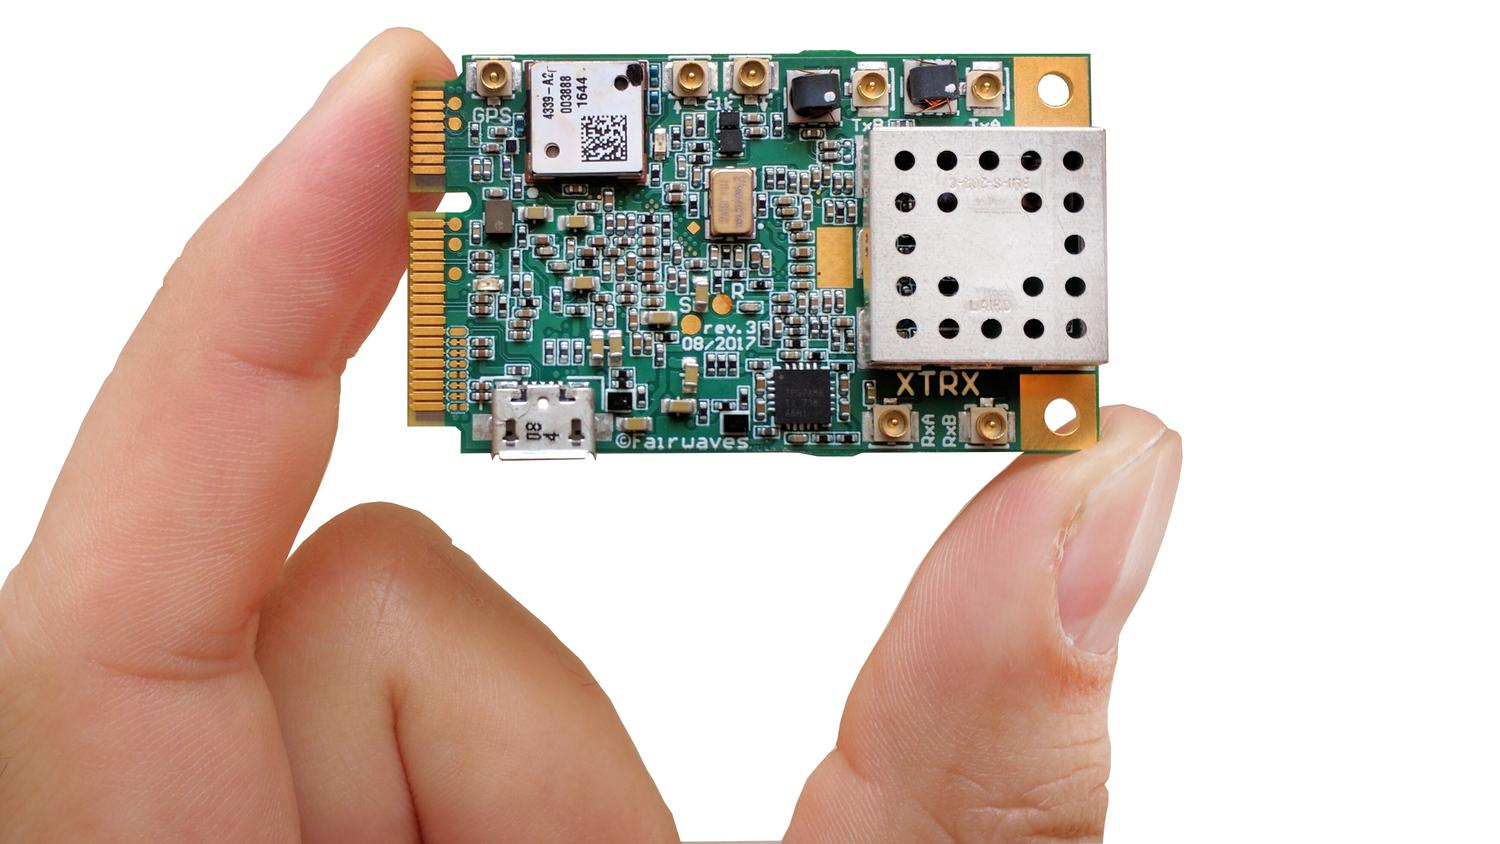
\includegraphics[width=0.9\textwidth]{templates/images/chapter06/xtrx-hand.jpg}
    \caption{XTRX Pro Board for Scale. Source: \cite{xtrx-io}}
    \label{fig:xtrx-io}
\end{figure}

Devices like the XTRX SDR shown in Figure \ref{fig:xtrx-io} integrate the full RF, analog and digital signal chain onto a single CMOS device. Devices like the LMS7002M focus on very low power consumption small form factor SDR applications such as UAV data links and handheld communication systems. This opens up a new design potential for a different suite of applications where using wideband waveforms or occupying noncontiguous spectrum can now be implemented in a much smaller form factor. The XTRX offers a 2x2 MIMO configuration with a stable clock accurate enough for cellular standards, an onboard GPS disciplined oscillator (GPSDO) and a SIM card reader. When inserted into an appropriate Mini PCIe slot, it appears as a USB SIM card reader, able to interface with a wide variety of single board computers such as the one used in our usecase.

\newpage
\section{Leveraging new streaming protocols}

%\begin{figure}[H]
%    \centering
%    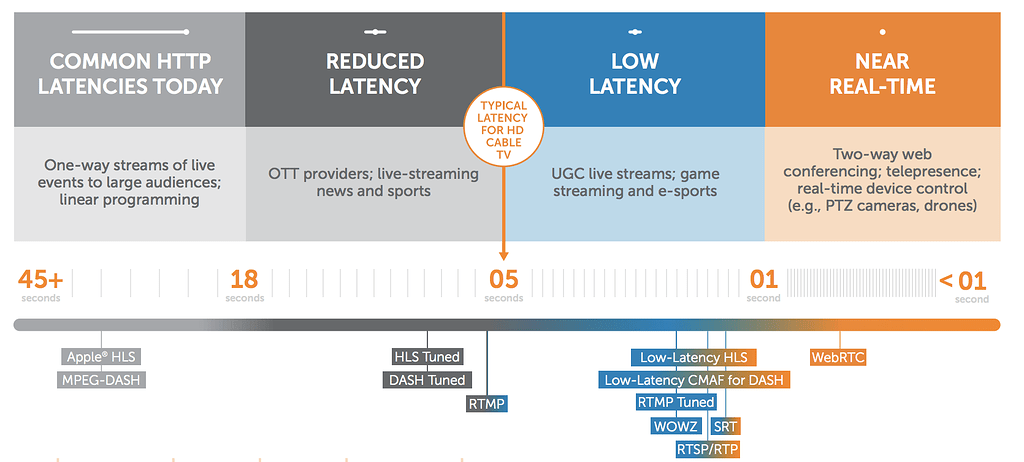
\includegraphics[width=\textwidth]{templates/images/chapter06/latency-comparison.png}
%    \caption{. Source: [*]}
%    \label{fig:board-diagram}
%\end{figure}
%https://www.wowza.com/blog/streaming-protocols

Traditional streaming protocols, such as RTSP and RTMP, support low-latency streaming. But they aren’t supported on all endpoints and work best for streaming to a small audience from a dedicated media server. These protocols achieve this by transmitting the data using a firehose approach rather than requiring local caching.

WebRTC is a combination of standards, protocols, and JavaScript APIs created by the World Wide Web Consortium (W3C) that enables real-time communications, allowing browser applications to make calls without any plugins and designed primarily with latency in mind. Different bodies such as the Internet Engineering Task Force, created to standardize the used protocols with browser APIs have been working on this implementation. Users connecting via Chrome, Firefox, or Safari can communicate directly through their browsers — enabling sub-500 millisecond latency to more than 85\% of all installed browsers globally for real-time communications on the internet.

\begin{table}[!ht]
           \begin{threeparttable}
        \caption{Comparison Between Video Streaming Protocols in ms. Source: \cite{impl-analysis-rtsp}}
        \label{tab:video-stream-protocols}
        \setlength\tabcolsep{1pt} % make LaTeX figure out intercolumn spacing
        
        \begin{tabular*}{\columnwidth}{@{\extracolsep{\fill}} lllll}
        \toprule
              &Establishment  &Reception  &Client to Client&Client to Web\\
        %     \multicolumn{4}{c}{Accuracy (\%)} \\ 
        %\cmidrule{3-6}
        %     & & K3 & K6 & L1 & mean\tnote{c} \\
        \midrule
              \textbf{RTSP} &2304 ms & 2161 ms & 37.807 ms & -\\
        \addlinespace
             \textbf{WebRTC} &1835 ms &1709ms&8.072 ms & 5.112 ms \\
        \addlinespace
              \textbf{Skype} &-&-&-&11.646 ms\\
        \bottomrule
        \end{tabular*}
        
        \smallskip
        \scriptsize
           \end{threeparttable}
        \end{table}

In a relevant work \cite{impl-analysis-rtsp}, two video streaming platforms implementing the most commonly used video streaming protocols, RTSP and WebRTC, have been implemented in order to conclude which offers the best results in the scope of web real-time video streaming applications. The analysis includes different parameters, namely the connection establishment and stream reception time, critical factors in applications such as our usecase. The results of the experiments discussed suggest that the use of the WebRTC protocol offers a vastly improved performance over the others, as can be seen in Table \ref{fig:board-diagram}.

%The performance improvement of the WebRTC implementation with respect to the RTSP implementation could be related to the use of UDP in all communications by the WebRTC protocol, whereas, in the RTSP protocol, TCP is used for the control. On the other hand, RTSP does not drop video packets, while the WebRTC protocol can do it if necessary. Finally, for peer-to-peer communications, WebRTC sends the video directly to the other peer, while, in the case of RTSP, the video is sent to the server and the server sends it to the other peer. Moreover, the WebRTC streaming platform shows better results than the analysed streaming applications in the stream reception time and in the stream establishment time in all cases, which means that, taking these measurements into account, the implemented streaming platform offers a better QoS than the studied applications. From the experiments, it is concluded that significant improvements have been obtained in WebRTC over RTSP for both communication establishment time and package sending time. Moreover, the implemented systems have been compared with the most common commercial applications through two experiments. Therefore, at this point, it is possible to confirm that the use of the WebRTC protocol provides better QoE and QoS than other protocols, and that the implemented Direct WebRTC system offers good results, according to the performed experiments.

\newpage
\section{Going cloud native}

Cloud-native today is almost synonymous with containers orchestrated by Kubernetes.  It wasn’t always thus.  It’s perfectly possible to build something that is cloud-native in all respects other than running in containers – i.e. dynamically orchestratable stateless microservices running in VMs – and production deployments have demonstrated many of the benefits, particularly with regard to simple, rapid scaling of the system and the automation of lifecycle management operations such as software upgrades.  

%Originally released by Google as recently as July 2015, Kubernetes became the seed project of the Cloud Native Computing Foundation (CNCF), and rapidly eclipsed all the other container orchestration solutions that were out there at the time.  It is now available in multiple mature distros including Red Hat OpenShift and Pivotal Container Services, and is also offered as a service by all the major public cloud operators.  It’s the only game in town when it comes to deploying and managing cloud native applications.  And, for the first time, we have a genuinely common platform for running cloud applications across both private and public clouds.  This is hugely helpful to telcos who are starting to explore the possibility of hybrid clouds for NFV.

Drawing a parallelism to the ETSI NFV architecture, it essentially covers the Virtual Infrastructure Manager (VIM) and VNF Manager (VNFM) roles. In its VIM role, Kubernetes schedules container-based workloads and manages their network connectivity, including a kind of Load Balancer as a Service, making it easy to deploy scale-out microservices. In its VNFM role, Kubernetes can monitor the health of each container instance and restart any failed instance.  It can also monitor the relative load on a set of container instances that are providing some specific micro-service and can scale out (or scale in) by spinning up new containers or spinning down existing ones.  In this sense, Kubernetes acts as a Generic VNFM.  For some types of workloads, especially stateful ones such as databases or state stores, Kubernetes native functionality for lifecycle management is not sufficient. In NFV terms, it comprizes a standardized way of building Specific VNFMs. But the beauty of Kubernetes is that it can provide a common environment across all types of cloud infrastructures. In this way, Kubernetes allows us to achieve a unified strategy for NFV that is entirely compelling.

%    \begin{figure}[H]
%        \centering
%        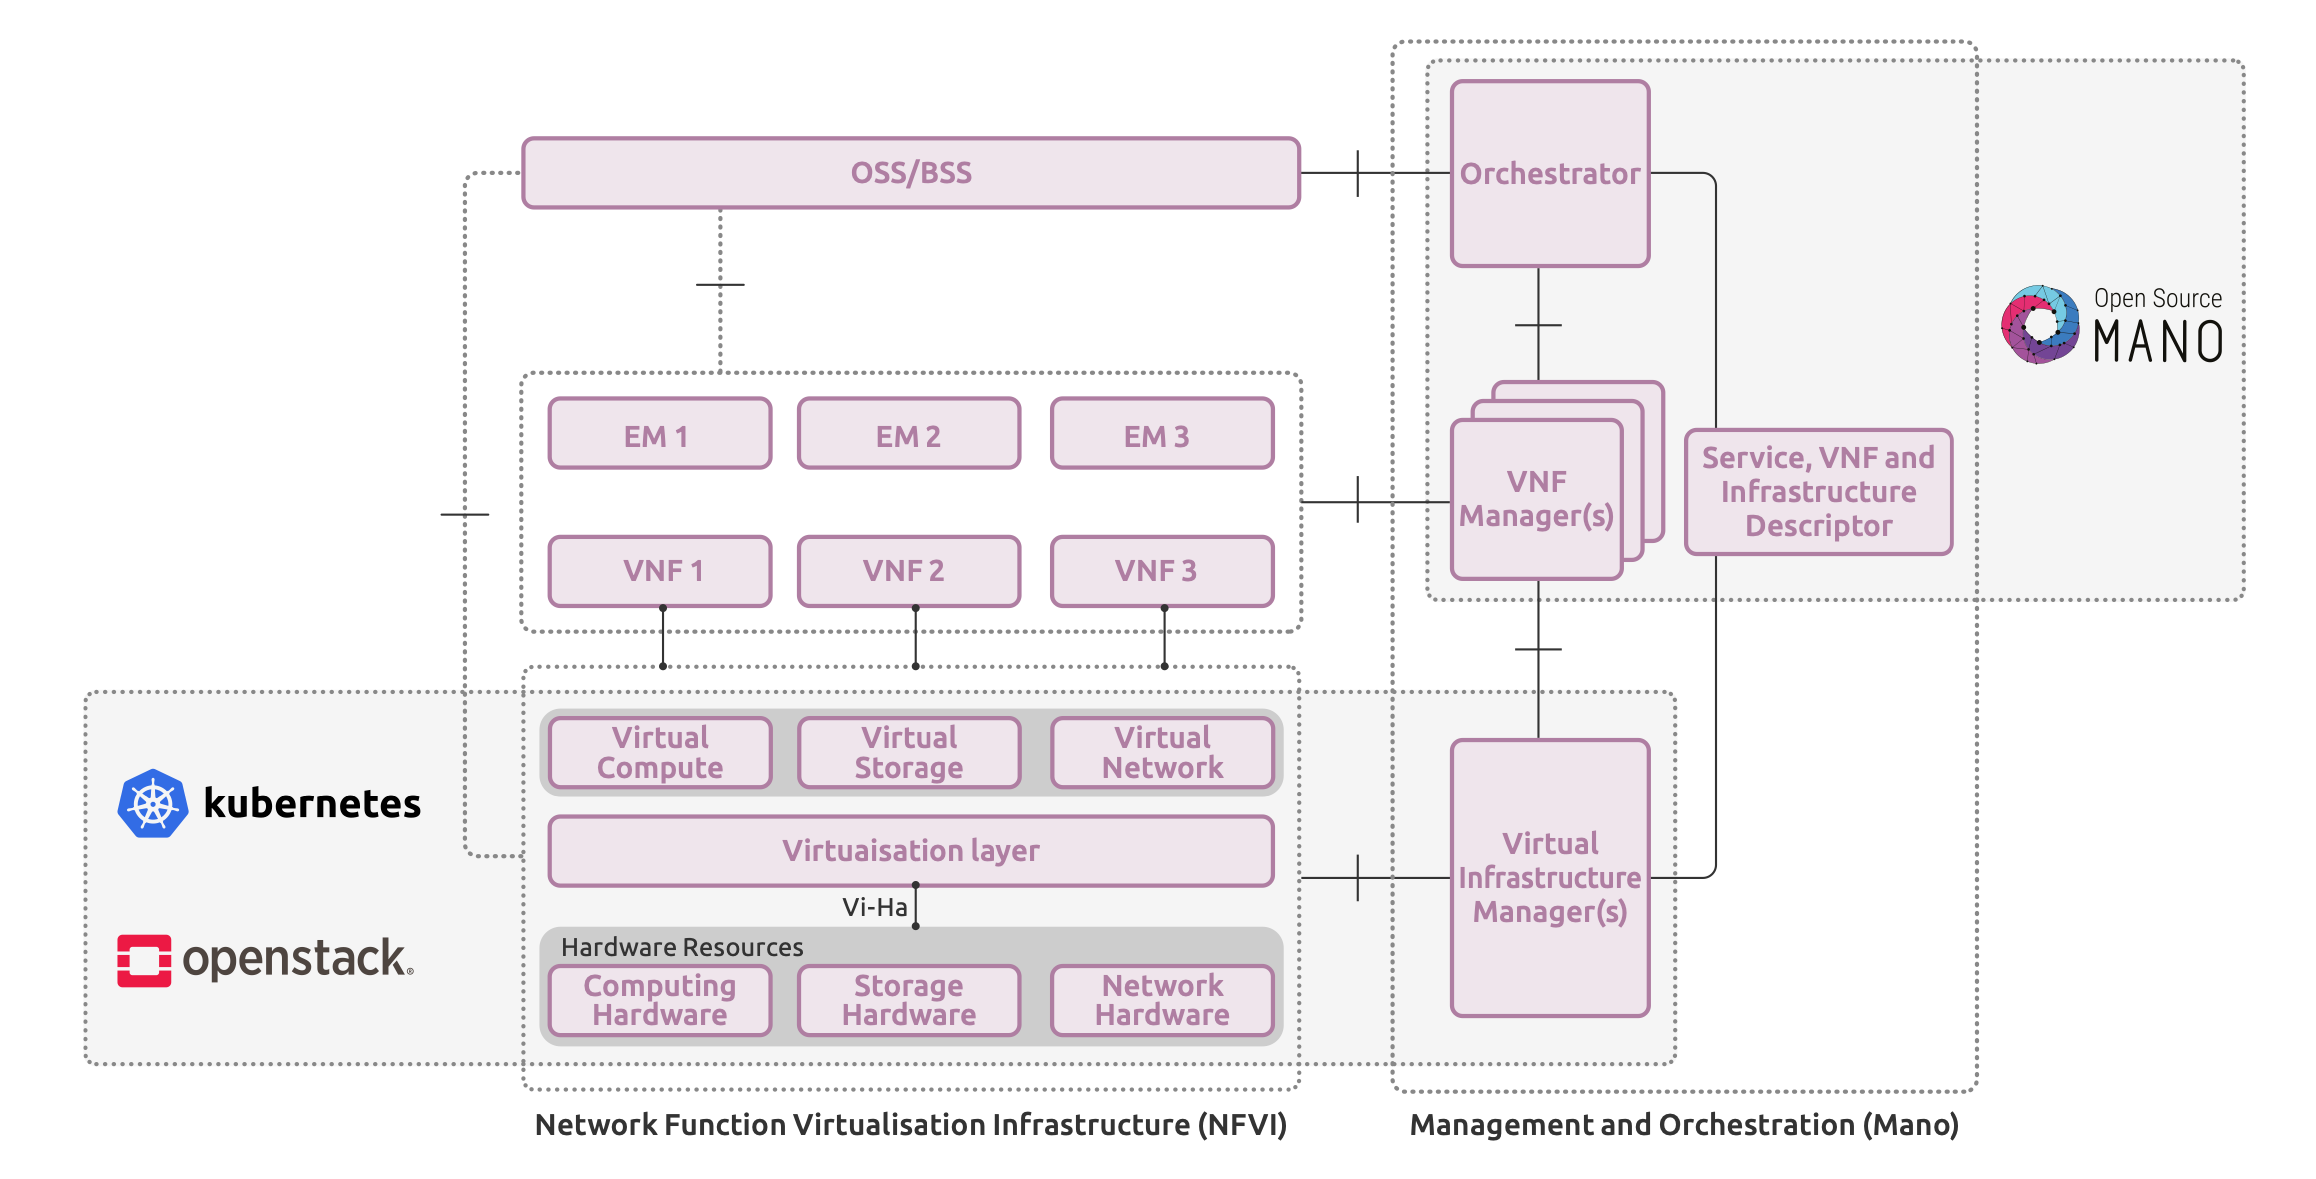
\includegraphics[width=0.9\textwidth]{templates/images/chapter06/kubernetes.png}
%        \caption{. Source: [*]}
%        \label{fig:board-diagram}
%    \end{figure}

%But Kubernetes goes way beyond the simple application lifecycle management envisaged by the ETSI NFV effort.  Kubernetes itself, together with a growing ecosystem of open source projects that surround it, is at the heart of a movement towards a declarative, version-controlled approach to defining both software infrastructure and applications.  The vision here is for all aspects of a complex cloud native system, including cluster infrastructure and application configuration, to be described in a set of documents that are under version control, typically in a Git repository, which maintains a complete history of every change.  These documents describe the desired state of the system, and a set of software agents act so as to ensure that the actual state of the system is automatically aligned with the desired state.  With the aid of a service mesh, changes to system configuration or software version can be automatically “canary” tested on a small proportion of traffic prior to be rolled out fully across the deployment.  If any issues are detected, the change can simply be rolled back. The high degree of automation and control offered by this kind of approach has enabled Web-scale companies to reduce software release cycles from months to minutes.

%This means today’s NFV infrastructure needs to be built on a hypervisor-based virtualization environment supporting VNFs deployed as virtual machines, with OpenStack acting as the VIM.  The conventional wisdom seems to be that you run Kubernetes on top of your existing VIM  and this is certainly possible: you just provision a number of VMs and treat these as hosts for the purposes of installing a Kubernetes cluster.  But then you end up with a two-tier environment in which you have to deploy and orchestrate services across some mix of cloud native network functions in containers and VM-based VNFs, where orchestration is driving some mix of Kubernetes, OpenStack or VMware APIs and where Kubernetes needs to coexist with proprietary VNFMs for life-cycle management. In our work with cloud-native VNFs, containers and Kubernetes, we’ve seen just how much easier it is to deploy and manage large scale applications using this approach compared with traditional hypervisor-based approaches.  The difference is huge.  We firmly believe that adopting this approach is the key to unlocking the massive potential of NFV to simplify operations and accelerate the pace of innovation in services. We think network operators should ratchet up the pressure on their vendors to deliver genuinely cloud native, container-based VNFs, and get serious about Kubernetes as an integral part of their NFV infrastructure.  Without any question, that is where the future lies.
%[https://www.metaswitch.com/blog/the-future-of-nfvi-is-kubernetes]

%\section{Closing Words}
%In October 2012, when a group of 13 network operators launched their white paper describing Network Functions Virtualization, the world of cloud computing technology looked very different than it does today.  As cloud computing has evolved, and as telcos have developed a deeper understanding of it, so the vision for NFV has evolved and changed out of all recognition. The early vision of NFV focused on moving away from proprietary hardware to software running on commercial off-the-shelf servers.  This was described in terms of “software appliances” and in describing the compute environment in which those would run, the NFV pioneers took their inspiration from enterprise IT practices of that era, which focused on consolidating servers with the aid of hypervisors that essentially virtualized the physical host environment.

%Meanwhile, hyperscale Web players were developing cloud-based system architectures that supported massive scalability with a high degree of resilience, which can be evolved very rapidly through incremental software enhancements, and can be operated very cost-effectively with the aid of a high degree of operations automation.  The set of practices developed by these players has come to be known as “cloud-native”, which can be summarized as dynamically orchestratable micro-services architectures, often based on stateless processing elements working with separate state storage micro-services, all deployed in Linux containers.

%It’s been clear to most network operators for at least a couple of years that cloud-native, microservices-based architectures is the right way to do NFV, for the following reasons:
%\begin{itemize}

%\item Promote rapid evolution of software capabilities to enable enhancement of services and operations, unlike legacy monolithic software architectures with their monthly upgrade cycles and their costly and complicated roll-out procedures.
%\item Enable independent and dynamic scaling of different functional elements of the system with active-active N+k redundancy, which minimizes the hardware resources required to deliver any given service.
%\item Software packaged in containers is inherently more portable than VMs and does much to eliminate the problem of complex dependencies between VMs and the underlying infrastructure which has been a major issue for NFV deployments to date.
%\item The cloud-native ecosystem includes some outstandingly useful open source projects. All of these combine to simplify, accelerate and lower the cost of developing, deploying and operating cloud-native network functions.
%\end{itemize}

%5G is the first new generation of mobile technology since the advent of the NFV era, and as such it represents a great opportunity to do NFV right – that is, the cloud-native way.  The 3GPP standards for 5G are designed to promote a cloud-native approach to the 5G core – but they don’t actually guarantee that 5G core products will be recognisably cloud-native.